\section{Theorie}
\label{sec:Theorie}
Ziel dieses Versuchs ist die Bestätigung der Quantennatur der Elektronenhüllen von Atomen.
Dazu werden Franck-Hertz-Kurven entnommen und untersucht.
\\
Das Franck-Hertz-Experiment gehört zu der Kategorie der Elektronenstoßexperimente. Dabei werden Atome mit Elektronen beschossen und der dabei auftretende Energieverlust der Elektronen
wird zur Auswertung genutzt. Daraus lassen sich Informationen über die Anregungsenergien der Energieniveaus herleiten.
In diesem Versuch werden beschleunigte Elektronen zur Anregung von Atomen im Quecksilberdampf genutzt. Es kommt zu elastischen und unelastischen Stößen mit den Quecksilberatomen.
Bei elastischen Stößen kommt es zu keiner Anregung, allein die Elektronenbewegungsrichtung verändert sich dabei aufgrund des ungleichen Masseverhältnisses von $\frac{m_e}{M}= 1836,201$.
Der abgegebene Energiebetrag 
\begin{equation}
    \symup{\Delta} E = \frac{4 m_0 M}{(m_0 + M)^2} E \approx \SI{1.1 e-5}{E}
\end{equation}
bei den elastischen Stößen ist vernachlässigbar. Die kinetische Energie der Elektronen wird dabei durch $E$ beschrieben.
\\
Erst ab erreichen einer bestimmten Elektronenenergie $E$ kommt es auch zu unelastischen Stößen. Die Elektronen der Geschwindigkeit $v_\text{vor}$ regen dabei die 
Quecksilberatome, die vereinfacht nach dem Bohrschen Atommodell betrachtet werden, in den ersten diskreten Zustand an und geben dabei die Energiedifferenz
\begin{equation}
    E_1-E_0 = \frac{m_0 v_\text{vor}^2}{2} - \frac{m_0 v_\text{nach}^2}{2}
\end{equation}
ab. Nach dem Stoß besitzen die Stoßelektronen die Geschwindigkeit $v_\text{nach}$ mit der Energie $E - (E_1 - E_0)$. Gemessen wird die Restenergie mit Hilfe von der Gegenfeldmethode.
Das angeregte Quecksilberatom geht mit einer Relaxationszeit in der Größenordnung $ \SI{10 e-8}{\second}$ in den Grundzustand zurück, wobei es ein Photon mit der Energie 
\begin{equation}
    h \nu = E_1 - E_0
\end{equation}
emittiert. Dabei ist $h$ das Plancksche Wirkungsquantun und $\nu$ die Frequenz der Lichtquelle.
Indem der Auffängerstrom $I_\text{A}$, in Abhängigkeit von der Beschleunigungsspannung $U_\text{B}$ gemessen wird, wird eine Franck-Hertz Kurve wie in Abbildung \ref{fig:id} zu sehen ist beobachtet. 
\begin{figure}
    \centering
    \caption{Idealisierter Zusammenhang zwischen Auffängerstrom $I_\text{A}$ und Beschleunigungsspannung $U_\text{B}$ beim Franck-Hertz-Experiment.\cite{v601}}
    \label{fig:id}
    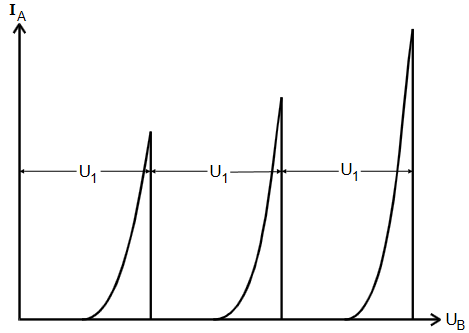
\includegraphics[width = 0.6 \textwidth]{pics/ideal.png}
\end{figure}
Da es noch weitere Einflüsse auf den Verlauf der Kurve gibt, auf die in \ref{subsec:einflüsse} eingegangen wird, ist die in Abbildung \ref{fig:id} zu sehende Kurve nur eine idealisierte Darstellung.
Es ist zu erkennen dass der Auffängerstrom $I_\text{A}$ bei steigender Beschleunigungsspannung $U_\text{B}$ ansteigt, bis $E$ für unelastische Stöße der Elektronen mit den Hg-Atomen ausreicht. Danach fällt $I_\text{A}$ direkt auf 0.
Wird $U_\text{B}$ weiter erhöht steigt der Strom wieder an, bis die Energie $2E$ erreicht ist. Dann reicht die Energie um jeweils zwei elastischen Stößen der Elektronen mit den Hg-Atomen zuzulassen. Dies
wiederholt sich bei steigender Beschleunigungsspannung bis hin zu mehreren Anregungen.
Die Spannungsdifferenzen zweier aufeinander folgender Maxima
\begin{equation}
    \symup{\Delta}U= \frac{1}{e_0} (E_1- E_0)
\end{equation}
ist gleich dem 1.Anregungspotential des Hg-Atoms.

\subsection{Einflüsse auf die Gestalt der Franck-Hertz-Kurve}
\label{subsec:einflüsse}

Die gemessene Kurve hat aufgrund einiger Nebeneffekte eine etwas andere Gestalt als die in Abbildung \ref{fig:id} angegebene.

\subsubsection{Einfluss des Kontaktpotentials}

Das tatsächliche Beschleunigungspotential ist von dem angelegten Beschleunigungspotential
verschieden, wenn die Elektroden aus Materialien bestehen, welche eine unterschiedliche Austrittsarbeit für Elektronen besitzen.
Da am Glühdraht ein Material mit kleinerer Austrittsarbeit $\Phi_\text{G}$ als die Austrittsarbeit $\Phi_\text{B}$ der Beschleunigungselektrode verwendet wird, um schon bei relativ niedriger Temperatur hohe Emissionsraten zu erzielen, wird auch hierbei
das Beschleunigungspotential verschoben. 
\begin{figure}
    \centering
    \caption{Potentialverhältnisse zwischen Glühkathode und Beschleunigungselektrode.\cite{v601}}
    \label{fig:verh}
    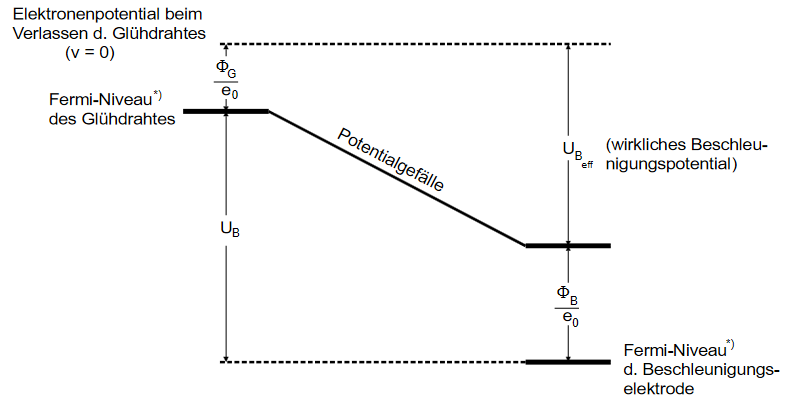
\includegraphics[width = 0.6 \textwidth]{pics/potdif.png}
\end{figure}
Das Potentialverhältniss ist in Abbildung \ref{fig:verh} zu sehen. Dabei hat das wirkliche Beschleunigungspotential $U_\text{B, eff}$ den Wert
\begin{equation}
    U_\text{B, eff}= U_\text{B} - K
\end{equation}
wobei $K = \sfrac{1}{e_0} (\Phi_\text{B}-\Phi_\text{G})$ das Kontaktpotential ist. Es folgt also dass die Franck-Hertz-Kurve um den Wert $K$ verschoben ist.

\subsubsection{Einfluss der Fermi-Dirac-Verteilung}

Die Annahme, dass die durch den Glühelektrischen Effekt emittierten Elektronen einen diskreten Energiebetrag haben, ist unzutreffend.
Da die Leitungselektronen im Innern eines Metalles bereits ein Energie-Spektrum besitzen, welches auch als Fermi-Dirac-Verteilung bezeichnet wird, treten sie bei der
Glühemission mit unterschiedlichen Anfangsgeschwindigkeiten aus der Metalloberfläche aus. Dies führt dazu, dass beim Duchlaufen des Beschleunigungspotentials $U_\text{B, eff}$ die Elektronen
bereits ein Energiespektrum besitzen. Dieses beginnt bei $U_\text{B, eff}$ und erstreckt sich mit schnell abnehmender Wahrscheinlichkeit zu höheren Energien hin. 
Die unelastischen Stöße treten also nicht nur bei diskreten Beschleunigungsspannungen auf, sondern erstrecken sich über einen endlichen Spannunsbereich. 
Die Franck-Hertz-Kurve wird daher ihren Anstieg in der Nähe eines Maximums verringern und danach nicht mehr unstetig auf den Wert 0 abfallen, sondern sich stetig dem
Stromminimum nähern. 

\subsubsection{Einfluss der elastischen Stöße}

Wie vorher erwähnt kommt es bei elastischen Stößen zu Richtungsänderungen der Elektronen, jedoch nur zu einer vernachlässigbaren Energieabnahme der Elektronen.
Geschehen elastische Stöße im Raum zwischen Kathode und Beschleunigungselektrode, wird die Franck-Hertz-Kurve nicht wesentlich verändert.
Kommt es jedoch zu elastischen Stößen zwischen Beschleunigungs- und Auffängerelektrode, führt die Richtungsänderungen zu einer Verteilung der z-Komponente der Geschwindigkeit.
Da der Auffängerstrom im Gegenfeldbereich von $v_z$ abhängt, führt auch dieser Effekt zu einer Abflachung und Verbreiterung der Kurve.

\subsubsection{Der Einfluss des Dampfdruckes}

Bei einer bestimmten Dampfdichte kommt es zu den erwarteten Messwerten. Ist die Dampfdichte jedoch zu klein, kann es auch bei sehr großer $U_\text{B}$ nur vereinzelt
zu Anregungen kommen, da de Stoßwahrscheinlichkeit klein ist. Bei sehr hohen Dampfdichten spielt der Energieverlust der elastischen Stöße eine immer größere Rolle, da es viel häufiger zu
diesen Stößen kommt.

\subsection{Der Versuchsaufbau und die Gegenfeldmethode}

Der Versuchsaufbau ist in Abbildung \ref{fig:auft} dargestellt.
\begin{figure}
    \centering
    \caption{Prinzipieller Aufbau des Franck-Hertz-Versuches.\cite{v601}}
    \label{fig:auft}
    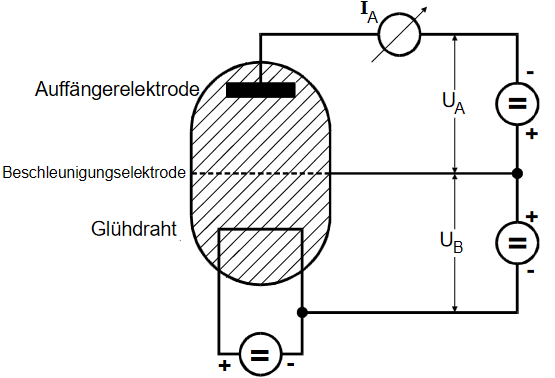
\includegraphics[width = 0.6 \textwidth]{pics/auft.png}
\end{figure}
In einem evakuierten Gefäß wird ein winziger Tropfen Quecksilber verdampft. Des weiteren sind in dem Gefäß eine Glühkathode, eine Beschleunigungsgitteranode und
eine Auffängerelektrode eingefasst. 
\\
Aus der Glühkathode werden Elektronen emittiert, welche durch die Beschleunigungsspannung $U_\text{B}$ zur Gitteranode hin beschleunigt werden.
Die kinetische Elektronenenergie wird mittels
\begin{equation}
    \frac{m_0 v_\text{vor}^2}{2} = e_0 \cdot U_\text{B}
\end{equation}
bestimmt. Die Bremsspannung $U_\text{A}$ bremst die Elektronen im Gegenfeld.
Nur die Elektronen, welche eine kinetische Energie
\begin{equation}
    \frac{m_0 v_\text{z}^2}{2} \geq e_0 U_\text{A}
\end{equation}
besitzen, erreichen die Auffängerelektrode. Der Auffängerstrom $I_\text{A}$ wird gemessen und gibt an wie viele Elektronen nach den Stößen die Elektrode erreichen.
Durch Temperaturänderung lässt sich die Quecksilberdampfdichte regeln.